\begin{nestedsection}{CoDeR Model for Continuous Deductive Reasoning}{model}
	CoDeR is an abstract model for continuous deductive reasoning over streamed RDF data that expresses the semantics of Continuous Datalog, thus supporting continuous reasoning expressed in both RIF-Core and OWL 2 RL.
	It is composed of a stream-based data model for expressing the streams $S$, $P$ and $N$ of each ${CDP = \{A,S,R\} \vDash \{A',P,N\}}$, and a minimal algebra of stream-to-stream operators for expressing the persistent set of axiomatic rules $A$.
	It casts the problem of applying those rules to streamed RDF data as that of iterative pattern matching, in a manner inspired by the Rete pattern matching algorithm \citep{forgy79}, though it is meant to support any such algorithm rather than prescribing one itself.

	% Stream-based Data Model
	\begin{nestedsection}{Data Model}{model: data}
		The data model of CoDeR is composed of two classes of streams: \emph{input}/\emph{output} streams and \emph{inter-operator} streams.

		In the first case, input/output streams provide the semantics of the streams $S$, $P$ and $N$ for any ${CDP}$ expressed by a CoDeR-based system.
		These streams are sequences of instances of RDF graphs compatible with the ongoing work on query semantics by the RSP working group\footnote{\url{https://github.com/streamreasoning/RSP-QL/blob/master/Semantics.md}};
		an instance of an RDF graph is an RDF graph annotated with the time interval for which it is valid \citep{SemanticStreamingManagement,sparkwave} according to the ${CDP}$ expressed: ${\langle \{(s,p,o),\dots,(s',p',o')\},i_{e},i_{n} \rangle}$.
		As the atomic units of Continuous Datalog are instances of facts, being triples in RDF, graph instances arriving on the streams $S$ must be translated into sequences of fact instances using the graph-to-triple operator described in \refsec{model: algebra}, where each fact instance inherits the valid time interval of the graph instance in which it originated.
		This interval, for any entailed graph/fact instance, is derived from the valid time intervals of the fact instances that justify it, as shown in \reffig{intersected-intervals}, being the graphical representation of valid times for transitive data continuously entailed by the ${CDP = \{\{c\,\text{:-}\,a,b\,.\},S,3\}}$ over instants ${i = 1 \dots 4}$:
		\begin{figure}[t]
			\centering
			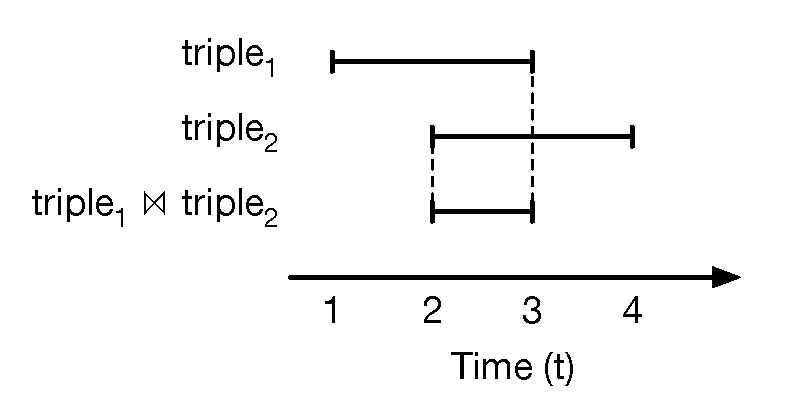
\includegraphics[width=0.45\textwidth]{intersected-intervals}
			\caption{Derivation of valid-time for entailed fact instance from those of its justifying fact instances.}
			\labelfig{intersected-intervals}
		\end{figure}
		\begin{align*}
			CDP_{1} & = \{c\,\text{:-}\,a,b\,.\} \cup \{ a \, . \} & \vDash & \{ c\,\text{:-}\,a,b\,. \, a \, . \} \\
			CDP_{2} & = \{c\,\text{:-}\,a,b\,.\} \cup \{ a \, . \, b \, . \} & \vDash & \{ c\,\text{:-}\,a,b\,. \, a \, . \, b \, . \, c \, . \} \\
			CDP_{3} & = \{c\,\text{:-}\,a,b\,.\} \cup \{ a \, . \, b \, . \} & \vDash & \{ c\,\text{:-}\,a,b\,. \, a \, . \, b \, . \, c \, . \} \\
			CDP_{4} & = \{c\,\text{:-}\,a,b\,.\} \cup \{ b \, . \} & \vDash & \{ c\,\text{:-}\,a,b\,. \, b \, . \}
		\end{align*}
		It is in the base case of this derivation that the semantic window range $R$ of a ${CDP}$ is expressed:
		each graph instance arriving on an input stream has a valid interval from the time of its arrival at the system for a duration equal to the range $R$.

		In the second case, inter-operator streams are produced and consumed by the stream-to-stream operators of CoDeR's minimal algebra.
		These streams are sequences of the intermediate results of processing between steps in the production of entailments.
		As the production of entailments in CoDeR is cast as a pattern matching problem, all intermediate results of this process will also take the form of instances of RDF graphs;
		for a given inter-operator stream, each such RDF graph will match the same graph pattern, that being a sub-pattern of the body of one of the axiomatic rules $A$.
		In addition, the continuous partial results for each specific graph pattern will occur in exactly one logical stream within a system, meaning that some logical streams may have multiple sources and/or multiple sinks within the system.
		As these instances of RDF graphs may be considered to be ``entailed'' by the presence of valid instances of their constituent RDF triples within the system, the same semantics of validity may be applied to these intermediate matches as to the true entailments of the model found on output streams, and their valid-time intervals may derived from their justifying instances in the same manner.
		It follows that inter-operator streams are functionally the same as input/output streams, only being distinct in their semantics:
		the former are sequences of homogeneous RDF graphs that hold no value outside of a system, while the latter contain heterogeneous graphs that are the entailments of either the system or its predecessor in the stream pipeline.

		Given that the ordering of instances in the output stream of a CoDeR-based system by the value of $i_{e}$ yields the sequence of instances in the semantic stream $P$ entailed by a ${CDP}$, and that their ordering by the value of $i_{n}$ yields the sequence of instances in the semantic stream $N$, this gives the output streams of CoDeR a dual semantics with respect to Continuous Datalog.
		Furthermore, this dual semantics applies to all the streams of CoDeR, each expressing both the stream of entailment instances \emph{and} instance negations produced by a specific pipeline of CoDeR operators applied to some set of continuous RDF data sources.
	\end{nestedsection}

	% Minimal Algebra
	\begin{nestedsection}{Minimal Algebra}{model: algebra}
		The minimal algebra of CoDeR is based on that of Positive Datalog, that being ${\{\bot, \text{:-}, \wedge\}}$.
		Of these, $\text{:-}$ and $\wedge$ may be expressed as stream-to-stream operators, the former being trivially incremental and the latter being the window-join \citep{ReteDBMS}, in order to support forward-chaining processing of fixed rules;
		$\bot$ is not an operator, but a special class of value represented in CoDeR by the ${rif\text{:}error()}$ class from RIF \citep{w3crif}).
		Further, in order to support both fixed-plan pattern-matching algorithms such as the Rete algorithm \citep{forgy79} and adaptive algorithms such as the Eddies algorithm \citep{eddies} and its derivatives \citep{CACQ,TCQ}, CoDeR replaces the window-join operator with the State Module of Eddies, algebraically represented by ${{}_b\Join_p}$.
		In addition to $\text{:-}$ and $\wedge$, CoDeR utilises a pair of stream-filter operators, $\sigma_{triple}$ and $\sigma_{external}$, for identifying \emph{basic patterns} as defined in SPARQL \citep{w3csparql} and the datatype functions of RIF-Core \citep{w3crifcore}.
		Finally, as basic patterns match individual triples, the CoDeR algebra includes a graph-to-triples operator ${{}_g\pi_t}$ to translate streams $S$ from the streams of graphs recommended by the RSP community to the streams of triples on which $\sigma_{triple}$ operate.
		In summary, the minimal algebra of CoDeR consists of the set of operators ${\{\text{:-}, {}_b\Join_p, \sigma_{triple}, \sigma_{external}, {}_g\pi_t\}}$.

		\begin{description}
			\item[$\sigma_{triple}$] \hfill \\
				The \emph{basic pattern match} of SPARQL is one-pass, and so is trivially interpreted as the stream-to-stream operator $\sigma_{(s,p,o)}$.
				It takes a stream of triple instances as input and produces a stream of triple instances that contains a subset of those instances in the input stream, maintaining the ordering of those instances.
				The contents of the produced stream are characterised as those triple instances from the input stream whose triples match the basic pattern ${(s,p,o)}$.
			\item[$\sigma_{external}$] \hfill \\
				This operator encompasses all of the one-pass built-in datatype functions of RIF-Core, and is also trivially interpreted as a stream-to-stream operator $\sigma_{f(a_1,\dots,a_n)}$, where each ${a_1,\dots,a_n}$ is either a variable or a constant value.
				It filters instances from its single input stream to a stream of instances that contains a subset of those instances in the input stream, maintaining the ordering of those instances.
				This filtering is based not on the semantic structure of the data but directly on the values of variables, which are consistent throughout any given graph pattern, thus the $\sigma_{external}$ operator expresses an \emph{advanced} component of an \emph{advanced graph pattern};
				as such, the contents of the produced stream are characterised as those graph instances from the input stream whose graphs match a specific advanced graph pattern.
		\end{description}
	\end{nestedsection}

%	\subimport{conclusions/}{future-work.tex}
\end{nestedsection}